% \chapter{Localization}
\chapter{定位}
\label{chap:localization}

% Robots employ sensors and actuators that are subject to uncertainty. Chapter \ref{chap:uncertainty} describes how to quantify this uncertainty using probability density functions that associate a probability with each possible outcome of a random process, such as the reading of a sensor or the actual physical change of an actuator. 

机器人采用有不确定性的传感器和驱动器。第\ref{chap:uncertainty}章描述了如何使用将概率与随机过程的每个可能结果相关联的概率密度函数对这种不确定性进行量化,例如传感器的读数或驱动器的实际物理变化。

%% Was Commented
%One of the most common probability density functions is the Gaussian distribution. It has the shape of a bell and can entirely be described by its mean --- the center of the bell curve --- and its variance, the width of the bell curve. 
%% Was Commented

% A possible way to localize a robot in its environment is to extract high-level features (Chapter \ref{chap:feature_extraction}), such as the distance to a wall from a number of different sensors. As the underlying measurements are uncertain, these measurements will be subject to uncertainty. How to calculate the uncertainty of a feature from the uncertainty of the sensors that detect this feature, is covered by the error propagation law. The key insight is that the variance of a feature is the weighted sum of all contributing sensors' variances, weighed by their impact on the feature of interest. This impact can be approximated by the derivative of the function that maps a sensor's input to the measurement of the feature. 

在环境中定位机器人的一种方法是提取高级特征(第\ref{chap:feature_extraction}章),例如从多个不同传感器到墙的距离。由于基础的测量不确定,这些测量将会受到不确定性的影响。如何从检测到该特征的传感器的不确定性计算特征的不确定性,由误差传播定律解决。关键的见解是,特征的方差是所有贡献传感器的方差的加权和,由它们对兴趣特征的影响而加权。这种影响可以由将传感器输入映射到特征测量的函数的导数近似。

%  Unfortunately, uncertainty keeps propagating without the ability to correct measurements. The goals of this chapter is to present mathematical tools and algorithms that will enable you to actually shrink the uncertainty of a measurement by combining it with additional observations.  In particular, this chapter will cover

不幸的是,不确定性不断传播,而无法纠正测量。本章的目标是提供数学工具和算法,使你能够通过将测量结果与其他观测结合在一起来减少测量的不确定性。特别地,本章将介绍


\begin{itemize}
% \item Using landmarks to improve the accuracy of a discrete position estimate (Markov Localization)
% \item Approximating continuous position estimates (Particle Filter)
% \item Optimal sensor fusion to estimate a continuous position estimate (Extended Kalman Filter)

\item 使用地标来提高离散位置估计的准确性(马尔可夫定位)
\item 近似连续位置估计(粒子滤波器)
\item 最优传感器融合来估计连续位置(扩展卡尔曼滤波)
\end{itemize}

% \section{Motivating Example}
% Imagine a floor with three doors, two of which are closer together, and the third farther down the corridor (Figure \ref{fig:three_door_example}). Imagine that your robot is able to detect doors, i.e., is able to tell whether it is in front of a wall or in front of a door. Such features can serve the robot as a landmark. Given a map of this simple environment and no information whatsoever where our robot is located, we can use landmarks to drastically reduce the space of possible locations once the robot has passed one of the doors. One way of representing this belief is to describe the robot's position with three Gaussian distributions, each centered in front of  a door and its variance a function of the uncertainty with which the robot can detect a door's center. (This approach is known as a multi-hypothesis belief.) What happens if the robot continues to move? From the error propagation law we know:

\section{动机示例}
想象一下有三个门的楼层,其中两个相互靠近,第三个更靠近走廊(如图\ref
{fig:three_door_example})。
想象一下,你的机器人能够检测到门,即能够判断是在墙前还是门前。
这样的特征可以作为机器人的地标。
给定这个简单环境的地图,并且没有任何机器人所在位置的信息,一旦机器人通过其中一个门,我们就可以使用地标大大减少可能位置的空间。
表示这种可能性的一种方式是用三个高斯分布描述机器人的位置,每个高斯分布的中心在门前,其方差是机器人可以检测门的中心的不确定性的函数。
(这种方法被称为多假设信念\todo{multi-hypothesis belief})。如果机器人继续移动会发生什么?
从误差传播定律我们知道:

\begin{enumerate}
% \item The Gaussians describing the robot's 3 possible locations will move with the robot.
% \item The variance of each Gaussian will keep increasing with the distance the robot moves.

\item 描述机器人3个可能位置的高斯将与机器人一起移动。
\item 每个高斯的方差随着机器人移动的距离而不断增加。
\end{enumerate}

% What happens if the robot arrives at another door? Given a map of the environment, we can now map the three Gaussian distributions to the location of the three doors. As all three Gaussians will have moved, but the doors are not equally spaced, only some of the peaks will coincide with the location of a door. Assuming we trust our door detector much more than our odometry estimate, we can now remove all beliefs that do not coincide with a door. Again assuming our door detector can detect the center of a door with some accuracy, our location estimate's uncertainty is now only limited by that of the door detector.

如果机器人到达另一扇门会怎么样?给定一个环境的地图,我们现在可以将三个高斯分布映射到三个门的位置。由于所有三个高斯将会移动,但是门并不是等间隔,只有一些山峰与门的位置一致。假设我们相信门检测器远远超过测距估计,现在可以删除与门不符的所有信念。再次假设门检测器可以以一定的精度检测到门的中心,位置估计的不确定性现在只受到门检测器的不确定性的限制。

% Things are just slightly more complicated if our door detector is also subject to uncertainty: there is a chance that we are in front of a door, but haven't noticed it. Then, it would be a mistake to remove this belief. Instead, we just weight all beliefs with the probability that there could be a door. Say our door detector detects false-positives with a 10\% chance. Then, there is a 10\% chance to be at any location that is not in front of door, even if our detector tells us we are in front of a door. Similarly, our detector might detect false-negatives with 20\% chance, i.e., tell us there is no door even though the robot is just in front of it. Thus, we would need to weigh all locations in front of a door with 20\% chance and all locations not in front of a door with 80\% likelihood if our robot tells us there is no door, even if we are indeed in front of one.

如果我们的门检测器也有不确定性,事情就会更复杂一些:我们有一次在门前,但没有注意到。那么,删除这个信念是错误的。相反,我们只是以可能有门的可能性来衡量所有的信念。比如说我们的门检测器以$10\%$的几率检测到假阳性。那么,即使检测器告诉我们机器人在门前,也有$10\%$的机会在除门前以外的任何位置。类似地,检测器以$20\%$的概率检测到假阴性,即表示,即使机器人正好位于前面,也没有检测到门。因此,如果我们的机器人告诉我们没有门,即使我们确实在门前,我们也需要给所有门的位置$20\%$,所有不是门位置$80\%$。

\begin{figure}
	\centering
		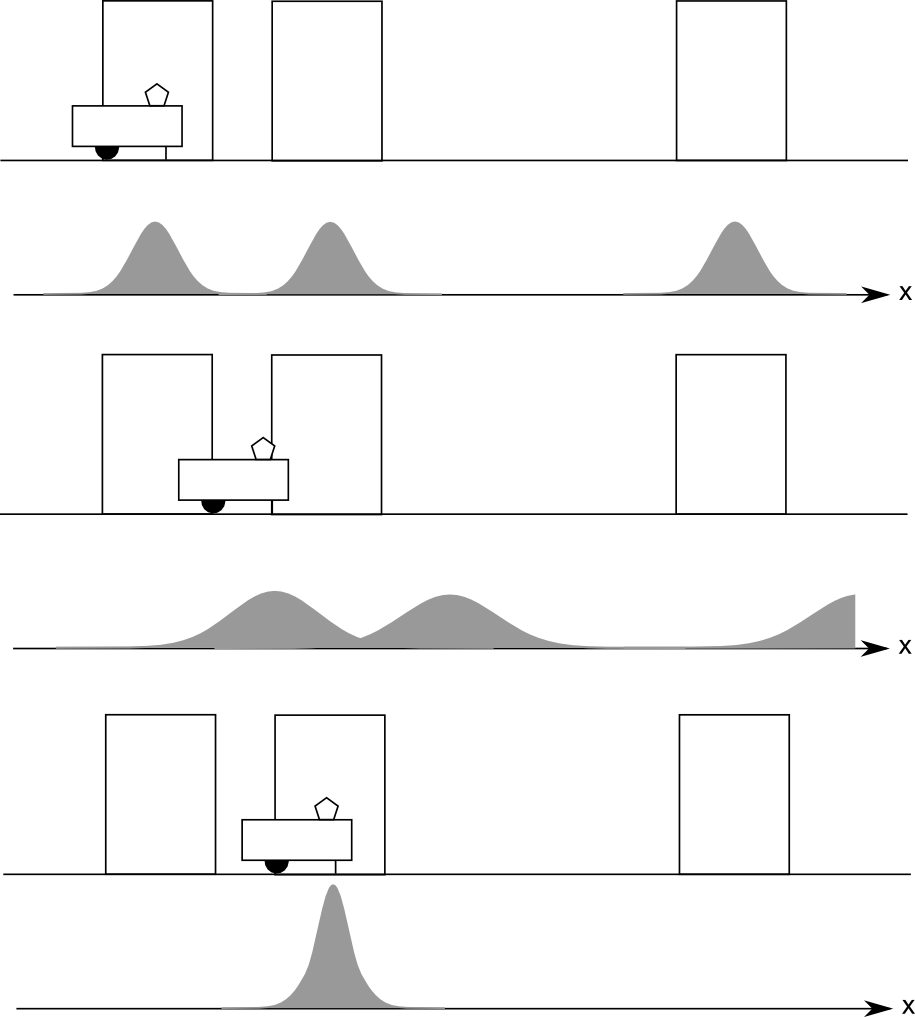
\includegraphics[width=\textwidth]{figs/three_door_example}
	% \caption{A robot localizing itself using a ``door detector'' in a known map. Top: Upon encountering a door, the robot can be in front of any of the three doors. Middle: When driving to the right, the Gaussian distributions representing its location also shift to the right and widen, representing growing uncertainty. Bottom: After detecting the second door, the robot can discard hypotheses that are not in front of the door and gains certainty on its location. }
	\caption{在已知地图中使用“门检测器”定位机器人。上:遇到门时,机器人可以在三个门中的任何一个前面。中:向右驾驶时,表示其位置的高斯分布也向右移动并且变宽,表示不确定性增加。下:检测到第二扇门后,机器人可以排除不在门前的假设,并增加其位置估计的确定性。}
	\label{fig:three_door_example}
\end{figure}

% \section{Markov Localization}\label{sec:markovloc}
% Calculating the probability to be at a certain location given the likelihood of certain observations is nothing else as a conditional probability. There is a formal way to describe such situations: Bayes' Rule (Section \ref{sec:bayesrule})\index{Bayes' rule}:

\section{马尔可夫定位}\label{sec:markovloc}
 给定某些观测的可能性,计算在某个位置处的概率其实就是一个条件概率。有一种正式的方式来描述这种情况:贝叶斯规则(见第\ref{sec:bayesrule}节)\index{贝叶斯规则}:

\begin{equation}
P(A|B)=\frac{P(A)P(B|A)}{P(B)}
\end{equation}

% \subsection{Perception Update}
% How does this map into a Localization framework? Lets assume, event $A$ is equivalent to be at a specific location $loc$. Lets also assume that event $B$ corresponds to the event to see a particular feature $feat$. We can now rewrite Bayes' rule to

\subsection{感知更新}
如何将贝叶斯规则用到定位的框架中呢?假设事件$A$相当于机器人在某个特定位置$loc$。也假设事件$B$对应于观测到特定特征$feat$的事件。我们现在可以重写贝叶斯规则:


\begin{equation}
P(loc|feat)=\frac{P(loc)P(feat|loc)}{P(feat)}
\end{equation}

% Rephrasing Bayes' rule in this way, we can calculate the probability to be at location $loc$, given that we see feature $feat$. This is known as \emph{Perception Update}\index{Perception Update (Markov Localization)}. For example, $loc$ could correspond to door 1, 2 or 3, and $feat$ could be the event of sensing a door. What do we need to know to make use of this equation?

以这种方式重述贝叶斯规则,我们可以计算观测到特征$feat$时机器人在位置$loc$的概率。这被称为\emph{感知更新(Perception Update)}\index{感知更新(Perception Update)(马尔科夫定位)})。例如,$loc$可以对应于门1、2或3,并且$feat$可以是感知到门的事件。我们需要哪些知识来使用这个方程呢?

\begin{enumerate}
% \item We need to know the prior probability to be at location loc $P(loc)$
% \item We need to know the probability to see the feature at this location $P(feat|loc)$
% \item We need the probability to encounter the feature feat $P(feat)$

\item 我们需要知道在位置$loc$的先验概率$P(loc)$
\item 我们需要知道在位置$loc$观测到特征的概率$P(feat|loc)$
\item 我们需要观测到特征$feat$的概率$P(feat)$
\end{enumerate}

% Lets start with (3), which might be the most confusing part of information we need to collect. The answer is simple, no matter what $P(feat)$ is, it will cancel out as the probability to be at any of the possible locations has to sum up to 1. (A simpler, although less accurate, explanation would be that the probability to sense a feature is constant and therefore does not matter.)

让我们从(3)开始,这可能是我们需要收集的最令人困惑的信息。答案很简单,无论$P(feat)$是什么,它都将被抵消,因为在任何可能的位置的概率总和必为1。(更简单但不太准确的解释是感知到特征的概率是恒定的,因此无关紧要。)

% The prior probability to be at location  $loc$, $P(loc)$, is called the \index{Belief Model} \emph{belief model}. In the case of the 3-door example, it is the value of the Gaussian distribution underneath the door corresponding to $loc$. 

在位置$loc$的先验概率$P(loc)$称为\emph{信念模型(Belief Model)}\index{信念模型(Belief Model)}。在前面3个门的例子中,它对应于$loc$的门下方的高斯分布的值。

% Finally, we need to know the probability to see the feature $feat$ at location $loc$ $P(feat|loc)$. If your sensor were perfect, this probability is simply 1 if the feature exists at this location, or 0 if the feature cannot be observed at this location. If your sensor is not perfect, $P(feat|loc)$ corresponds to the likelihood for the sensor to see the feature if it exists.

最后,我们需要知道在位置$loc$处观测到特征$feat$的概率$P(feat|loc)$。如果你的传感器是完美的,如果特征存在于该位置,则该概率为1,如果该位置不能观测到该特征,则为0。如果你的传感器不完美,则$P(feat|loc)$对应于如果特征存在,传感器观测到该特征的可能性。

% The final missing piece is how to best represent possible locations. In the graphical example in Figure \ref{fig:three_door_example} we assumed Gaussian distributions for each possible location. Alternatively, we can also discretize the world into a grid and calculate the likelihood of the robot to be in any of its cells. In our 3-door world, it might make sense to choose grid cells that have just the width of a door.

最后是如何最好地表示可能的位置。在图\ref{fig:three_door_example}的图形示例中,我们假设每个可能位置都是高斯分布。或者,我们还可以将世界离散成一个网格,并计算机器人处于其任何单元格中的可能性。在三个门的例子中,选择宽度与门相同的网格单元可能是有意义的。

% \subsection{Action Update}
% One of the assumptions in the above thought experiment was that we know with certainty that the robot moved right. We will now more formally study how to treat uncertainty from motion. Recall, that odometry input is just another sensor that we assume to have a Gaussian distribution; if our odometer tells us that the robot traveled a meter, it could have traveled a  little less or a little more, with decreasing likelihood. We can therefore calculate the posterior probability of the robot moving from a position $loc'$ to $loc$ given its odometer input $odo$:

\subsection {动作更新}
上述实验中的一个假设是我们确定地知道机器人向右移动。我们现在更正式地研究如何处理运动的不确定性。回想一下,里程计的输入只是我们假设具有高斯分布的另一个传感器;如果我们的里程表告诉我们,机器人行进了一个米,它可能是少一点,或多一点,可能性逐渐降低。因此,给定里程表输入$odo$,我们可以计算机器人从位置$loc'$移动到位置$loc$的后验概率:

\begin{equation}
P(loc'->loc|odo)=P(loc'->loc)P(odo|loc'->loc)/P(odo)
\end{equation}

% This is again Bayes' rule. The unconditional probability $P(loc'->loc)$ is the prior probability for the robot to have been at location $loc'$. The term $ P(odo|loc'->loc)$ corresponds to the probability to get odometer reading $odo$ after traveling from a position $loc'$ to $loc$. If getting a reading of the amount $odo$ is reasonable for the distance from $loc'$ to $loc$ this probability is high. If its unreasonable, for example if the distance is much larger than the robot could possibly ever have driven, this probability should be very low. 

这也是贝叶斯规则。无条件概率$P(loc'->loc)$是机器人曾位于$loc'$的先验概率。$P(odo|loc'->loc)$对应于从位置$loc'$移动到$loc$后里程表读数为$odo$的概率。如果从$loc'$到$loc$的距离中读取$odo$的数量是合理的,那么这个概率会很高。如果它不合理,例如如果距离远远大于机器人可能会前进的距离,这个概率应该非常低。

% As the robot's location is uncertain, the real challenge is now that the robot could have potentially been everywhere to start with. We therefore have to calculate the posterior probability $P(loc|odo)$ for all possible positions $loc'$. This can be accomplished by summing over all possible locations:

由于机器人的位置不确定,现在真正的挑战在于机器人的潜在起点是任意的。因此,我们必须为所有可能的位置$loc'$计算后验概率$P(loc|odo)$。这可以通过对所有可能的位置求和来实现:

\begin{equation}
P(loc|odo)=\sum_{loc'}P(loc'->loc)P(odo|loc'->loc)
\end{equation}

% In other words, the law of total probability requires us to consider all possible locations the robot could have ever been at. This step is known as \emph{Action Update}\index{Action Update (Markov Localization)}. In practice we don't need to calculate this for all possible locations, but only those that are technically feasible given the maximum speed of the robot. We note also that the sum notation technically corresponds to a convolution (Section \ref{sec:convolution}) of the probability distribution of the robot's location in the environment with the robots odometry error probability distribution.

换句话说,总概率的定律要求我们考虑机器人曾经的所有可能的位置。此步骤称为\emph{动作更新(Action Update)}\index{动作更新(Action Update)(马尔科夫定位)}。实际中,我们不需要计算所有可能的位置,而只计算给定机器人最大速度的情况下在技术上可行的位置。我们还注意到,求和符号技术上对应于环境中机器人位置的概率分布的卷积,其中环境中有机器人里程计误差概率分布\todo{to improve}(见第\ref{sec:convolution}节)。

% \subsection{Summary and Examples}
% We have now learned two methods to update the belief distribution of where the robot could be in the environment. First, a robot can use external landmarks to update its position. This is known as \emph{perception update} in  and relies on exterioception. Second, a robot can observe its internal sensors. This is known as \emph{action update} and relies on proprioception. The combination of action and perception updates is known as \emph{Markov Localization}\index{Markov Localization}. You can think about the action update to increase the uncertainty of the robot's position and the perception update to shrink it. (You can also think about the action update as a discrete version of the error propagation model.) Also here we are using the robotics kinematic model and the noise model of your odometer to calculate $ P(odo|loc'->loc)$.

\subsection{小结和示例}
我们现在已经学到了两种方法来更新机器人在环境中位置的信念分布。首先,机器人可以使用外部地标来更新其位置。这被称为\emph{感知更新},依赖于体外感知。第二,机器人可以观测其内部传感器。这被称为\emph{动作更新},依赖于本体感知。动作更新和感知更新的组合称为\emph{马尔科夫定位}\index{马尔科夫定位(Markov Localization)}。你可以认为动作更新增加机器人位置的不确定性,而感知更新缩小机器人位置的不确定性。(你还可以将动作更新看成误差传播模型的离散版本。)此外,我们还使用机器人运动学模型和里程表的噪声模型来计算$P(odo|loc'->loc)$。

% \paragraph{Example 1: Topological Map}
% This example describes one of the first successful real robot systems that employed Markov Localization in an office environment. The experiment is described in more detail in a 1994 article of AI Magazine. The office environment consisted of two rooms and a corridor that can be modeled by a topological map\index{Topological Map} (Figure \ref{fig:dervish_example}). In a topological map, areas that the robot can be in are modeled as vertices, and navigable connections between them are modeled as edges of a graph. The location of the robot can now be represented as a probability distribution over the vertices of  this graph.

\paragraph{示例1:拓扑图}
该示例描述了在办公环境中成功使用马尔可夫定位的真正机器人系统之一。在AI杂志的1994年文章更详细地描述该实验。办公室环境包括两个房间和一个走廊,可以通过拓扑图\index{拓扑图}(图\ref{fig:dervish_example})建模。在拓扑图中,机器人可以达到的区域被建模为顶点,它们之间的可导航连接被建模为图的边。机器人的位置现在可以表示为该图顶点上的概率分布。

\begin{figure}
	\centering
		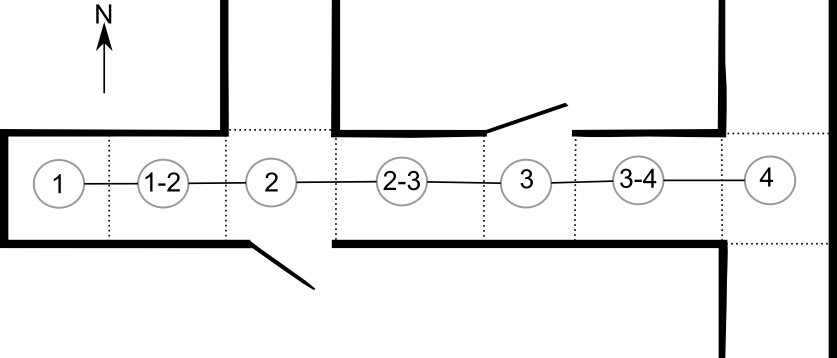
\includegraphics[width=\textwidth]{figs/dervish_example}
	% \caption{An office environment consisting of two rooms connected by a hallway. A topological map is super-imposed.}
	\caption{一个由走廊连接的两个房间组成的办公环境。拓扑图叠加其上。}
	\label{fig:dervish_example}
\end{figure}

% The robot has the following sensing abilities:

机器人具有以下感知能力:

\begin{itemize}
% \item It can detect a wall to its left or right.
% \item It can detect an open door to its left or right.
% \item It can detect a closed door to its left or right.
% \item It can detect whether it is an open hallway.

\item 它可以检测到左侧或右侧的墙壁。
\item 它可以检测到其左侧或右侧的打开的门。
\item 它可以检测到其左侧或右侧的关闭的门。
\item 它可以检测是否是一个开放的走廊。
\end{itemize}

% Unfortunately, the robot's sensors are not at all reliable. The researchers have experimentally found the probabilities to obtain a certain sensor response for specific physical positions using their robot in their environment. These values are provided in Table \ref{tab:dervish_example}. 

不幸的是,机器人的传感器完全不可靠。研究人员已经通过实验发现了使用机器人在其环境中为特定物理位置获得特定传感器响应的概率。这些值见表\ref{tab:dervish_example}。

\begin{table}
\footnotesize
\begin{tabular}{lccccc}
 	& 墙壁	& 关闭的门 & 打开的门	& 走廊 & 门厅\\
\hline
无检测	& 70\%	& 40\%&	5\%	& 0.1\% & 30\%\\
检测到关闭的门 & 30\% &	60\%& 0\% &0\%	& 5\%\\
检测到打开的门 & 0\%	& 0\%&	90\% & 10\% & 15\%\\
检测到走廊 & 0\% &	 0\%&	0.1\% & 90\% &50\%\\
\hline
\end{tabular}
\normalsize
% \caption{Conditional probabilities of the Dervish robot detecting certain features in the Stanford laboratory.\label{tab:dervish_example}}
\caption{斯坦福大学实验室Dervish机器人检测某些特征的条件概率。
\label{tab:dervish_example}}
\end{table}

% For example, the success rate to detect a closed door is only 60\%, whereas a foyer looks like an open door in 15\% of the trials. This data corresponds to the conditional probability to detect a certain feature given a certain location.

例如,检测到关闭的门的成功率只有$60\%$,而在$15\%$的实验中,门厅被认为是打开的门。该数据对应于给定一定位置时检测到特定特征的条件概率。

% Consider now the following initial belief state distribution: $p(1-2)=0.8$ and $p(2-3)=0.2$. Here, $1-2$ etc.\ refers to the position on the topological map in Figure \ref{fig:dervish_example}. You know that the robot faces east with certainty. The robot now drives for a while until it reports ``open hallway on its left and open door on its right''. This actually corresponds to location 2, but the robot can in fact be anywhere. For example there is a 10\% chance that the open door is in fact an open hallway, i.e.\ the robot is really at position 4. How can we calculate the new probability distribution of the robot's location? Here are the possible trajectories that could happen:

现在考虑以下初始信念状态分布:$p(1-2)=0.8$和$p(2-3)=0.2$。这里,$1-2$ 指的是图\ref{fig:dervish_example}中的拓扑图上的位置。你确切知道机器人面向东方。机器人现在行驶一段时间,直到它报告“左边是走廊,右边是打开的门”。这实际上对应于位置2,但机器人实际上可能在任何地方。例如,有$10\%$的概率是打开的门实际上是一个走廊,即机器人位于位置4。我们该如何计算机器人位置的新概率分布?以下是可能的轨迹:

% The robot could move from $2-3$ to $3$, $3-4$ and finally $4$. We have chosen this sequence as the probability to detect an open door on its right is zero for $3$ and $3-4$, which leaves position $4$ as the only option if the robot has started at $2-3$. In order for this hypothesis to be true, the following events need to have happened, their probabilities are given in parentheses:

机器人可以从$2-3$移动到$3$、$3-4$最后$4$。我们选择这个序列,因为在$3$和$3-4$检测到右边是打开的门的概率为0,如果机器人从$2-3$开始,那么$4$是唯一选择。要使这个假设为真,以下事件需要发生,他们的概率在括号中给出:

\begin{enumerate}
% \item The robot must have started at $2-3$ (20\%)
% \item Not have seen the open door at the left of $3$ (5\%) and not have seen the wall at the right (70\%)
% \item Not have seen the wall to its left (70\%) and not have seen the wall to its right (70\%) at node $3-4$
% \item Correctly identify the open hallway to its left (90\%) and mistake the open hallway to its right for an open door (10\%)

\item 机器人从$2-3$($20\%$)开始
\item 在位置$3$,没有检测到左边的打开的门($5\%$),没有检测到右边的墙壁($70\%$)
\item 在位置$3-4$没有检测到左边的墙壁($70\%$),没有检测到右边的墙壁($70\%$)
\item 正确检测到左边的走廊($90\%$),错误的把右边的走廊看成打开的门($10\%$)
\end{enumerate}

% Together, the likelihood that the robot got from position $2-3$ to position $4$ is therefore given by $0.2*0.05*0.7*0.7*0.7*0.9*0.1=0.03\%$, that is very unlikely.

因此,机器人从$2-3$到$4$的可能性是$0.2*0.05*0.7*0.7*0.7*0.9*0.1=0.03\%$,表明这个可能性很低。

% The robot could also move from $1-2$ to $2$, $2-3$, $3$, $3-4$ or $4$. We can evaluate these hypotheses in a similar way:

机器人也可以从$1-2$移动到$2$、$2-3$、$3$、$3-4$和$4$。我们可以用类似的方式评估这些假设:

\begin{itemize}
% \item The chance that it correctly detects the open hallway and door at position $2$ is $0.9*0.9$, so the chance to be at position $2$, having started at $1-2$, is $0.8*0.9*0.9=64\%$.
% \item The robot cannot have ended up at position $2-3$, $3$, and $3-4$ because the chance of seeing an open door instead of a wall on the right side is zero in all these cases.
% \item In order to reach position $4$, the robot must have started at $1-2$ has a chance of $0.8$. The robot must not have seen the hallway on its left and the open door to its right when passing position $2$. The probability for this is $0.001*0.05$. The robot must then have detected nothing at $2-3$ ($0.7*0.7$), nothing at $3$ ($0.05*0.7$), nothing at $3-4$ ($0.7*0.7$), and finally mistaken the hallway on its right for an open door at position $4$ ($0.9*0.1$). Multiplied together, this outcome is very unlikely.

\item 在位置$2$,它正确地检测到走廊和门的概率是$0.9*0.9$,所以,从$1-2$开始,位置为$2$的概率为$0.8*0.9*0.9=64\%$。
\item 机器人不能在位置$2-3$、$3$和$3-4$终止,因为在所有这些情况下,检测到右边是打开的门而不是墙壁的概率为零。
\item 为了到达位置$4$,机器人必须从$1-2$开始,概率为$0.8$。机器人在通过位置$2$时,几乎不可能检测到左边是走廊、右边是打开的门,概率为$0.001*0.05$。那么机器人在$2-3$什么都没检测到($0.7*0.7$),在位置$3$什么都没检测到($0.05*0.7$),在位置$3-4$什么都没检测到($0.7*0.7$),最后在位置$4$误将右边的走廊认为是打开的门($0.9*0.1$)。全部相乘,这个假设是不大可能的。
\end{itemize}

% Given this information, we can now calculate the posterior probability to be at a certain location on the topological map by adding up the probabilities for every possible path to get there. 

给定这些信息,现在我们可以将每个可能路径的概率相加来计算在拓扑图上的某个位置的后验概率。

% \paragraph{Example 2: Grid-based Markov Localization}
\paragraph{示例2:基于网格的马尔可夫定位}

\begin{figure}
	\centering
		\includegraphics[width=\textwidth]{figs/markov_grid_example}
	% \caption{Markov localization on a grid. The left colum shows the likelihood to be in a specific cell as grey value (dark colors correspond to high likelihoods). The right column shows the actual robot location. Arrows indicate previous motion. Initially, the position of the robot is unknown, but recorded upwards motion makes positions at the top of the map more likely. After the robot has encountered a wall, positions away from walls become unlikely. After rightwards and down motions, the possible positions have shrunk to a small area.}
	\caption{网格上的马尔可夫定位。左列以灰度值表示机器人在特定单元格中的可能性(深色对应于高的可能性)。右列显示实际的机器人位置。箭头表示以前的动作。最初,机器人的位置是未知的,但记录到向上运动使得机器人位于地图上方的位置更可能。机器人遇到墙后,远离墙壁的位置变得不太可能。经过向右和向下的运动,可能的位置已经缩小到一个小区域。}
	\label{fig:markov_grid_example}
\end{figure}

% Instead of using a coarse topological map, we can also model the environment as a fine-grained grid. Each cell is marked with a probability corresponding to the likelihood of the robot being at this exact location (Figure \ref{fig:markov_grid_example}). We assume that the robot is able to detect walls with some certainty. The images in the right column show the actual location of the robot. Initially, the robot does not see a wall and therefore could be almost anywhere. The robot now moves northwards. The action update now propagates the probability of the robot being somewhere upwards. As soon as the robot encounters the wall, the perception update bumps up the likelihood to be anywhere near a wall. As there is some uncertainty associated with the wall detector, the robot cannot only be directly at the wall, but anywhere --- with decreasing probability --- close by. As the action update involved continuous motion to the north, the likelihood to be close to the south wall is almost zero. The robot then performs a right turn and travels along the wall in clockwise direction. As soon as it hits the east wall, it is almost certain about its position, which then again decreases.

我们还可以将环境建模为细粒度网格,而不是使用粗糙的拓扑图。每个单元被标记为机器人在位置的概率(图\ref{fig:markov_grid_example})。我们假设机器人能以某种可能性检测到墙壁。右栏中的图像显示机器人的实际位置。最初,机器人没有检测到墙壁,因此可以在几乎任何地方。现在机器人向北移动。动作更新将传播机器人在某处的概率。一旦机器人遇到墙壁,感知更新会增加靠近墙壁的可能性。由于墙壁探测器存在一些不确定性,机器人不仅可以直接在墙壁处,而且可以在附近(概率递减)。由于行动更新涉及到北部持续运动,靠近南墙的可能性几乎为零。然后机器人右转,顺时针方向沿着墙壁行进。一旦撞到东墙,几乎可以肯定它的位置,然后概率再次降低。

% \section{Particle Filter}
% Although grid-based Markov Localization can provide compelling results, it can be computationally very expensive, in particular when the environment is large and the resolution of the grid is small. This is in part due to the fact that we need to carry the probability to be at a certain location forward for every cell on the grid, regardless of how small this probability is. An elegant solution to this problem is the particle filter. It works as follows:

\section{粒子滤波器}
虽然基于网格的马尔科夫定位可以提供令人信服的结果,但是在计算上可能非常昂贵,特别是当环境较大并且网格的分辨率较小时。部分原因是我们需要记录机器人在网络上的每个单元格的概率,不管这个概率有多小。这个问题的一个优雅的解决方案是粒子滤波器。它的工作原理如下:

\begin{enumerate}
% \item Represent the robots position by N particles that are randomly distributed around its estimated initial position. For this, we can either use one or more Gaussian distributions around the initial estimate(s) of where the robot is, or choose an uniform distribution (Figure \ref{fig:particlefilter_example}).
% \item Every time the robot moves, we will move each particle in the exact same way, but add noise to each movement much like we would expect it the real robot to exhibit. Without a perception update, the particles will spread apart farther and farther.
% \item Upon a perception event, we evaluate every single particle using our sensor model. What would the likelihood be to have a perception event such as we observed at this location? We can then use Bayes' rule to update each particles position.
% \item Once in a while or during perception events that render certain particles infeasible, particles that have a too low probability can be deleted, while those with the highest probability can be replicated.

\item 用随机分布在估计的初始位置周围的$N$个粒子表示机器人的位置。为此,我们可以在机器人所在的初始估计周围使用一个或多个高斯分布,或使用均匀分布(图\ref{fig:particlefilter_example})。
\item 机器人每次移动时,我们将以完全相同的方式移动每个粒子,但是对每个运动添加噪声,就像我们期望真正的机器人会做的一样。没有感知更新,粒子将分散得越来越远。
\item 在感知事件之后,我们用传感器模型来评估每个粒子。有了感知事件后(比如我们该位置观测到的),可能性会怎么变呢?然后,我们可以使用贝叶斯规则来更新每个粒子的位置。
\item 在一段时间内或在使某些粒子不可行的感知事件期间,可以删除概率太低的粒子,同时可以复制概率最高的粒子。
\end{enumerate}

\begin{figure}
	\centering
		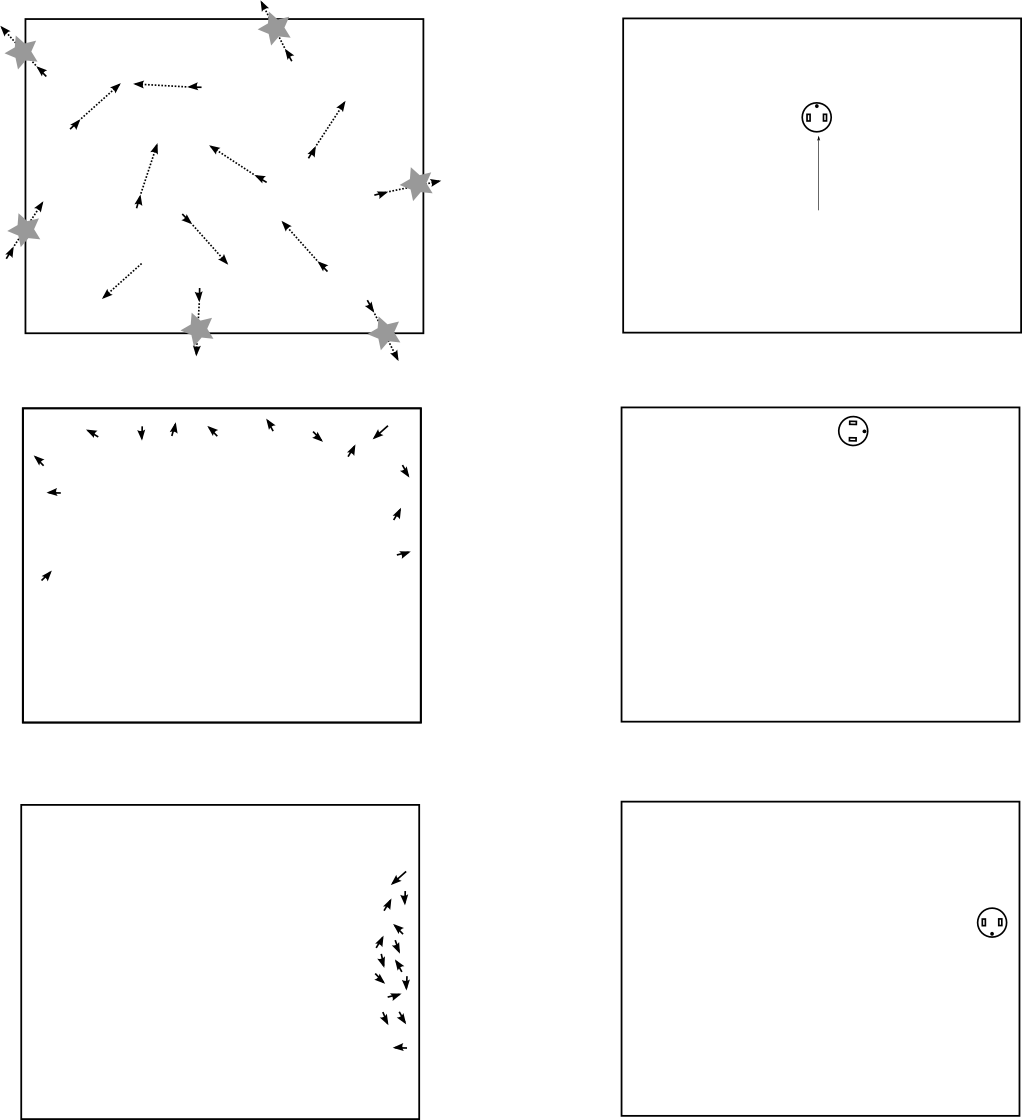
\includegraphics[width=\textwidth]{figs/particlefilter_example}
	% \caption{Particle filter example. Possible positions and orientations of the robot are initially uniformly distributed. Particles move based on the robot's motion model. Particles that would require the robot to move through a wall in absence of a wall perception event are deleted (stars). After a perception event, particles too far of a wall become unlikely and their positions are resampled in the vicinity of a wall. Eventually, the particle filter converges.}
	\caption{粒子滤波器示例。最初,机器人的可能位置和方向是均匀分布的。粒子根据机器人运动模型移动。在没有检测到墙壁的情况下,将使机器人移动通过墙壁的粒子删除(星星)。在感知到墙壁后,离墙壁太远的粒子变得不可能,在墙壁附近重新采样。最终,粒子滤波器收敛。}
	\label{fig:particlefilter_example}
\end{figure}

% \section{The Kalman Filter}
% The location of a robot is subject to uncertainty due to wheel-slip and encoder noise. We learned in the past how the variance in position can be derived from the variance of the robot's drive train using the error propagation law and the forward kinematics of the robot. One can see that this error is continuously increasing unless the robot has additional observations, e.g., of a static object with known location. This update can be formally done using Bayes' rule, which relates the likelihood to be at a certain position given that the robot sees a certain feature to the likelihood to see this feature at the hypothetical location. For example, a robot that drives towards a wall will become less and less certain of its position (action update) until it encounters the wall (perception update). It can then use its sensor model that relates its observation with possible positions. Its real location must be therefore somewhere between its original belief and where the sensor tells it to be. Bayes' rule allows us to perform this location for discrete locations and discrete sensor error distributions. This is inconvenient as we are used to represent our robot's position with a 2D Gaussian distribution. Also, it seems much easier to just change the mean and variances of this Gaussian instead of updating hundreds of variables. The goals of this section are

\section {卡尔曼滤波器}

由于车轮滑动和编码器的噪声,机器人的位置受到不确定性的影响。我们学习了如何使用误差传播定律和机器人的正向运动学,从机器人传动系的方差中推导出位置的方差。可以看到,除非机器人获得额外的观测(例如位置已知的静止物体),否则该误差不断增加。可以使用贝叶斯规则正式地完成此更新,贝叶斯规则把机器人检测到某特征时机器人在某一位置的概率和机器人在假定位置检测到该特征的概率联系到一起。例如,朝向墙壁行进的机器人将越来越不确定其位置(动作更新),直到遇到墙壁(感知更新)。然后可以使用其传感器模型将其观测与可能的位置相关联。因此,它的真实位置必定位于其原始信念与传感器所感知的位置之间。贝叶斯规则使我们在离散位置和离散传感器误差分布上实现定位。这是不方便的,因为我们习惯用二维高斯分布来表示我们的机器人的位置。而且,相对于更新数百个变量,改变这个高斯的平均值和方差似乎更容易。本节的目标是:

\begin{itemize}
% \item to introduce a technique known as the Kalman filter to perform action and perception updates exclusively using Gaussian distributions.
% \item to formally introduce the notion of a feature map.
% \item to develop an example that puts everything we learned so far together: forward kinematics, error propagation and feature estimation.

\item 引入一种称为卡尔曼滤波器的技术,仅使用高斯分布来执行动作更新和感知更新。
\item 正式介绍特征图的概念。
\item 用一个例子将我们至今所学到的都集中在一起:正向运动学、误差传播和特征估计。
\end{itemize}

% \subsection{Probabilistic Map based localization}
% In order to localize a robot using a map, we need to perform the following steps

\subsection{基于概率地图的定位}
为了使用地图定位机器人,我们需要执行以下步骤:

\begin{enumerate}
% \item Calculate an estimate of our new position using the forward kinematics and knowledge of the wheel-speeds that we sent to the robot until the robot encounters some uniquely identifiable feature.
% \item Calculate the relative position of the feature (a wall, a landmark or beacon) to the robot.
% \item Use knowledge of where the feature is located in global coordinates to predict what the robot should see.
% \item Calculate the difference between what the robot actually sees and what it believes it should see.
% \item Use the result from (4) to update its belief by weighing each observation with its variance.

\item 使用正向运动学和我们发送到机器人的车轮速度来估计新位置,直到机器人遇到一些唯一可识别的特征。
\item 计算特征(墙壁、地标或信标)到机器人的相对位置。
\item 使用全局坐标中特征位置的知识来预测机器人检测到什么。
\item 计算机器人实际检测和它认为检测的差。
\item 使用(4)的结果更新其信念,用每个观测的方差作为权重。
\end{enumerate}

% Steps 1-2 are based on the lectures on ``Forward Kinematics'' and ``Line detection''. Step 3 uses again simple forward kinematics to calculate the position of a feature stored in global coordinates in a map in robot coordinates. Step 4 is a simple subtraction of what the sensor sees and what the map says. Step 5 introduces the Kalman filter. Its derivation is involved, but its intuition is simple: why just averaging between where I think I am and what my sensors tell me, if my sensors are much more reliable and should carry much higher weight?

步骤1-2基于“正向运动学”和“直线检测”的讲座。步骤3再次使用简单的正向运动学来计算存储在地图中全局坐标系下的特征在机器人坐标系下的位置。步骤4是传感器检测内容和地图所说内容的简单相减。步骤5引入卡尔曼滤波器。它的推导比较复杂,但它的直观理解很简单:如果我的传感器更可靠,应该赋予更大的权重,为什么只对我觉得的和传感器告诉我的取均值呢?


% \subsection{Optimal Sensor Fusion}
% The Kalman filter is an optimal way to fuse observations that follow a Gaussian distribution. The Kalman filter has an update and a prediction step. The update step uses a dynamical model of the system (such as the forward kinematics of your robot) and the prediction step uses a sensor model (such as the error distribution calibrated from its sensors). The Kalman filter does not only update the state of the system (the robot's position) but also its variance. For this, it requires knowledge of all the variances involved in the system (e.g., wheel-slip and sensor error) and uses them to weigh each measurement accordingly. Before providing the equations for the Kalman filter, we will make use a simple example that explains what ``optimal'' means in this context.

\subsection{最优的传感器融合}
卡尔曼滤波器是融合符合高斯分布的观测值的最优方法。卡尔曼滤波器有更新和预测两步。更新步骤使用系统的动力学模型(例如你的机器人的正向运动学),预测步骤使用传感器模型(例如从其传感器校准的误差分布)。卡尔曼滤波器不仅可以更新系统的状态(机器人的位置),还可以更新其方差。为此,它需要系统中涉及的所有方差(例如,车轮滑动和传感器误差),然后用这些方差对每个观测赋予权重。在给出卡尔曼滤波器的方程之前,我们将使用一个简单的例子来解释在这个上下文中“最优”的意思。

% Let $ \hat{q_1}$ and $ \hat{q_2}$ be two different estimates of a random variable and $ \sigma^2_1$ and $ \sigma^2_2$ their variances, respectively. Let $ q$ be the true value. This could be the robot's position, e.g. The observations have different variances when they are obtained by different means, say using odometry for $ \hat{q_1}$ and by using the location of a known feature for $ \hat{q_2}$. We can now define the weighted mean-square error

令$\hat{q_1}$和$\hat{q_2}$是一个随机变量两个不同估计值,方差分别为$\sigma^2_1$和$\sigma^2_2$。令$q$为真实值。这可能是机器人的位置。当通过不同的方法获得时,观测值有不同的差异,例如使用里程计得到$\hat{q_1}$,使用已知特征的位置得到$\hat{q_2}$。我们现在可以定义加权均方误差:

 \begin{equation}
S=\displaystyle\sum_{i=1}^{n}\frac{1}{\sigma_i} (q-\hat{q_i})^2
\end{equation}

% that is, $ S$ is the sum of the errors of each observation $ \hat{q_i}$ weighted by its standard deviation $ \sigma_i$. Each error is weighted  with its standard deviation to put more emphasis on observations whose standard deviation is low. Minimizing  $S$ for $n=2$ yields the following optimal expression for $q$:

也就是说,$S$是按照标准差$\sigma_i$加权的观测值$\hat{q_i}$的误差总和。每个误差用其标准偏差加权,以更加重视标准偏差较小的观测值。$n=2$最小化$S$得到$q$的最优表达式:

\begin{equation}
q=\frac{\hat{q_1}\sigma_2^2}{\sigma_1^2+\sigma_2^2}+\frac{\hat{q_2}\sigma_1^2}{\sigma_1^2+\sigma_2^2}
\end{equation}

% or, equivalently,
或者等价地,

\begin{equation}
q=\hat{q_1}+\frac{\sigma_1^2}{\sigma_1^2+\sigma_2^2}(\hat{q_2}-\hat{q_1})\label{eq:optimalfusion}
\end{equation}

% We have now derived an expression for fusing two observations with different errors that provably minimizes the error between our estimate and the real value. As $q$ is a linear combination of two random variables (Section \ref{sec:lcombrandom}, the new variance is given by

现在我们已经推导出一个表达式,用于将误差不同的两个观测值融合,这可以使估计值与实际值之间的误差最小化。由于$q$是两个随机变量的线性组合(见第\ref{sec:lcombrandom}章),新的方差为:

\begin{equation}
\sigma^2=\frac{1}{\frac{1}{\sigma_1^2}+\frac{1}{\sigma_2^2}}
\end{equation}

% Interestingly, the resulting variance is smaller than both $\sigma_1$ and $\sigma_2$, that is, adding additional observation always helps reducing accuracy instead of introducing more uncertainty. 

有趣的是,由此产生的方差小于$\sigma_1$和$\sigma_2$,即引入额外的观测总是有助于提高\todo{typo in english version}准确性,而不是引入更多的不确定性。

% \subsection{Integrating prediction and update: The Kalman Filter}
% Although we have introduced the problem above as fusing two observations of the same quantity and weighing them by their variance, we can also interpret the equation above as an update step that calculates a new estimate of an observation based on its old estimate and a measurement. Remember step (4) from above: $ \hat{q_2}-\hat{q_1}$ is nothing else then the difference between what the robot actually sees and what it thinks it should see. This term is known as innovation in Kalman lingo. We can now 
% rewrite (\ref{eq:optimalfusion}) from above into

\subsection{对预测与更新积分:卡尔曼滤波器}
虽然我们已经将上述问题介绍为融合同一量的两个观测值,并通过其方差来加权,但我们也可以将上述方程解释为更新步骤,即利用旧估计和测量值来计算新估计。记住上面的步骤(4):$\hat{q_2}-\hat{q_1}$只不过是机器人实际看到的和它认为看到的差。这个术语被卡尔曼语言称为创新\todo{innovation, and a typo in `nothing else then'}。我们现在可以
重写(\ref{eq:optimalfusion})为:

\begin{equation}
\hat{x}_{k+1}=\hat{x}_k+K_{k+1}\tilde{y}_{k+1}
\end{equation}

% Here, $ \hat{x}_k$ is the state we are interested in at time $ k$, $ K_{k+1}=\frac{\sigma_1^2}{\sigma_1^2+\sigma_2^2}$ the Kalman gain, and $ \tilde{y}_{k+1}=\hat{q_2}-\hat{q_1}$  the innovation. Unfortunately, there are few systems that allow us to directly measure the information we are interested in. Rather, we obtain a sensor measurement $ z_k$ that we need to convert into our state somehow. You can think about this the other way round too and predict your measurement $ z_k$ from your state $ x_k$. This is done using the observation model $ H_k$, so that

这里,$\hat{x}_k$是我们感兴趣的在时间$k$的状态,$K_{k+1}=\frac{\sigma_1^2}{\sigma_1^2+\sigma_2^2}$为卡尔曼增益,$\tilde{y}_{k+1}=\hat{q_2}-\hat{q_1}$创新\todo{innovation}。不幸的是,几乎没有系统允许我们直接测量我们感兴趣的信息。而是获得一个传感器测量值$z_k$,我们需要转换成我们的状态。你可以通过另一种方式来思考这一点,从你的状态$x_k$中预测你的测量值$z_k$。这是使用观测模型$H_k$完成的,有:

\begin{equation}
\tilde{y}_{k}=z_k-H_k x_k
\end{equation}

% In our example $ H_k$ was just the identity matrix; in a robot position estimation problem $ H_k$ is a function that would predict how a robot would see a certain feature. As you can see, all the weighing based on variances is done in the Kalman gain $ K$.

在我们的例子中,$H_k$只是单位矩阵;在机器人位置估计问题中,$H_k$是预测机器人如何观测某个特征的函数。正如你所看到的,所有根据方差的赋予权重操作都是在卡尔曼增益$K$中实现的。

% The perception update step shown above, also known as prediction step is only half of what the Kalman filter does. The first step is the update step, which corresponds to the action update we already know. In fact, the variance update in the Kalman filter is exactly the same as we learned during error propagation. Before going into any more details on the Kalman filter, it is time for a brief disclaimer: the Kalman filter only works for linear systems. Forward kinematics of even the simplest robots are mostly non-linear, and so are observation models that relate sensor observations and the robot position. Non-linear systems can be dealt with the Extended Kalman Filter.

上面所示的感知更新步骤,也称为预测步骤只是卡尔曼滤波器的一半。第一步是更新步骤,这对应于我们知道的动作更新。事实上,卡尔曼滤波器的方差更新与我们在误差传播中讲到的完全一样。在讲解卡尔曼滤波器的更多细节之前,现在是一个简短的免责声明:卡尔曼滤波器仅适用于线性系统。即使最简单的机器人的正向运动学也大都是非线性的,将传感器观测和机器人位置相关联的观测模型也是非线性的。非线性系统可以用扩展卡尔曼滤波器来处理。

% \section{Extended Kalman Filter}\label{sec:EKF}
% In the extended Kalman filter, the state transition and observation models do not need to be linear functions of the state but may instead be differentiable functions. The action update step looks as follows:

\section {扩展卡尔曼滤波器} 
\label{sec:EKF}
在扩展卡尔曼滤波器中,状态转换和观测模型不需要是状态的线性函数,而可以是可微分的函数。动作更新步骤如下所示:

\begin{equation}
\hat{\boldsymbol{x}}_{k'|k-1} = f(\hat{\boldsymbol{x}}_{k-1|k-1}, \boldsymbol{u}_{k-1})
\end{equation}

% Here $ f()$ is a function of the old state $ \boldsymbol{x}_{k-1}$ and control input $ \boldsymbol{u}_{k-1}$. This is nothing else as the odometry update we are used to, where $ f()$ is a function describing the forward kinematics of the robot, $ \boldsymbol{x}_k$ its position and $ \boldsymbol{u}_k$ the wheel-speed we set.

% We can also calculate the covariance matrix of the robot position

这里$f()$是旧状态$\boldsymbol{x}_{k-1}$和控制输入$\boldsymbol{u}_{k-1}$的函数。这只是我们习惯的里程计更新,其中$f()$是描述机器人正向运动学的函数,$\boldsymbol{x}_k$为其位置,$\boldsymbol{u}_k$为我们设定的车轮速度。

我们还可以计算机器人位置的协方差矩阵:

\begin{equation}
\boldsymbol{P}_{k'|k-1} = \nabla_{x,y,\theta}f \boldsymbol{P}_{k-1|k-1}\nabla_{x,y,\theta}f^T + \nabla_{\Delta_{r,l}}f\boldsymbol{Q}_{k-1}\nabla_{\Delta_{r,l}}f
\end{equation}

% This is nothing else as the error propagation law applied to the odometry of the robot with $ \boldsymbol{Q}_k$ the covariance matrix of the wheel-slip and the Jacobian matrices of the forward kinematic equations $ f()$ with respect to the robot's position (indicated by the index $ x,y,\theta$) and with respect to the wheel-slip of the left and right wheel.

这只是把误差传播定律应用到机器人的里程计上,其中$\boldsymbol{Q}_k$是轮子滑动的协方差矩阵,正向运动学方程$f()$(相对于机器人的位置(由下标$x,y,\theta$表示)和左右轮的车轮滑移)的雅可比矩阵\todo{to improve}。

% The perception update (or prediction) step looks as follows:

感知更新(或预测)步骤如下:

\begin{eqnarray}
\hat{\boldsymbol{x}}_{k|k'} &=& \hat{\boldsymbol{x}}_{k'|k-1} + \boldsymbol{K}_{k'}\tilde{\boldsymbol{y}}_{k'}\\
\boldsymbol{P}_{k|k'} &=& (I - \boldsymbol{K}_{k'} {\boldsymbol{H}_{k'}}) \boldsymbol{P}_{k'|k-1}
\end{eqnarray}

% At this point the indices $ k$ should start making sense. We are calculating everything twice: once we update from $ k-1$ to an intermediate result $ k'$ during the action update, and obtain the final result after the perception update where we go from $ k'$ to $ k$.

在这一点上,下标$k$开始有意义。每样我们都计算两次:一次是在动作更新过程中从$k-1$更新到中间结果$k'$,另一次是从$k'$到$k$的感知更新之后得到最终结果。

% We need to calculate three additional variables:

我们需要计算三个附加变量:

\begin{enumerate}
% \item The innovation $ \tilde{\boldsymbol{y}}_{k}=\boldsymbol{z}_{k}-h(\hat{\boldsymbol{x}}_{k|k-1})$
% \item The covariance of the innovation $\boldsymbol{S}_{k}={\boldsymbol{H}_{k}}\boldsymbol{P}_{k|k-1}{\boldsymbol{H}_{k}^\top}+\boldsymbol{R}_{k}$
% \item The (near-optimal)  Kalman gain $ \boldsymbol{K}_{k}=\boldsymbol{P}_{k|k-1}{\boldsymbol{H}_{k}^\top}\boldsymbol{S}_{k}^{-1}$

\item 创新\todo{innovation}$\tilde{\boldsymbol{y}}_{k}=\boldsymbol{z}_{k}-h(\hat{\boldsymbol{x}}_{k|k-1})$
\item 创新的协方差$\boldsymbol{S}_{k}={\boldsymbol{H}_{k}}\boldsymbol{P}_{k|k-1}{\boldsymbol{H}_{ķ}^\top}+\boldsymbol{R}_{K}$
\item (近似最优)卡尔曼增益$\boldsymbol{K}_{k}=\boldsymbol{P}_{k|k-1}{\boldsymbol{H}_{k}^\top}\boldsymbol{S}_{K}^{-1}$
\end{enumerate}

% Here $ h()$ is the observation model and $ \boldsymbol{H}$ its Jacobian. How these equations are derived is involved (and is one of the fundamental results in control theory), but the idea is the same as introduced above: we wish to minimize the error of the prediction.

这里$h()$是观测模型,而$\boldsymbol{H}$则为其雅克比矩阵。这些方程的推导是复杂难懂的(并且是控制理论的基本结果之一),但是这个想法与上面介绍的相同:我们希望最小化预测的误差。

% \subsection{Odometry using the Kalman Filter}
% We will show how a mobile robot equipped with a laser scanner can correct its position estimate by relying on unreliable odometry, unreliable sensing, but a correct map, in an optimal way.
% Whereas the update step is equivalent to forward kinematics and error propagation we have seen before, the observation model and the ``innovation'' require additional steps to perform odometry. 

\subsection{使用卡尔曼滤波器的方程式}
我们将展示配备激光扫描仪的移动机器人是如何依靠不可靠的里程计、不可靠的感知,以最佳的方式来校正其位置估计的。
而更新步骤相当于我们以前看到的正向运动学和误差传播,观测模型和“创新”需要额外的步骤来执行里程计。

% \paragraph{1. Prediction Update}
% We assume for now that the reader is familiar with calculating $ \hat{\boldsymbol{x}}_{k'|k-1}=f(x,y,\theta)^T$ and its variance $ \boldsymbol{P}_{k'|k-1}$. Here, $ \boldsymbol{Q}_{k-1}$, the covariance matrix of the wheel-slip error,  is given by

\paragraph{1.预测更新}
我们假设读者熟悉$\hat{\boldsymbol{x}}_{k'|k-1}=f(x,y,\theta)^T$及其方差$\boldsymbol{P}_{K'|K-1}$的计算。这里,车轮滑动误差的协方差矩阵$\boldsymbol{Q}_{k-1}$为:

\begin{equation}
\boldsymbol{Q}_{k-1}=\left[\begin{array}{cc}k_r|\Delta s_r & 0\\0 & k_l|\Delta s_l|\end{array}\right]
\end{equation}

% where $ \Delta s$ is the wheel movement of the left and right wheel and $ k$ are constants. See also the odometry lab for detailed derivations of these calculations and how to estimate $ k_r$ and $ k_l$.  The state vector $ \boldsymbol{\hat{x}_{k'|k-1}}$ is a 3x1 vector, the covariance matrix $ \boldsymbol{P_{k'|k-1}}$ is a 3x3 matrix, and $ \nabla_{\Delta_{r,l}}$ that is used during error propagation is a 3x2 matrix. See the error propagation lecture for details on how to calculate $ \nabla_{\Delta_{r,l}}$.

其中$\Delta s$是左右轮的车轮运动,$k$是常数。有关这些计算的详细推导以及如何估计$k_r$和$k_l$,可以参考里程计实验。状态向量$\boldsymbol{\hat{x}_{k'|k-1}}$是$3\times 1$向量,协方差矩阵$\boldsymbol{P_{k'|k-1}}$是$3\times 3$矩阵,并且在误差传播期间使用的$\nabla_{\Delta_{r,l}}$是$3\times 2$矩阵。有关如何计算$\nabla_{\Delta_{r,l}}$的详细信息,请参阅误差传播讲义。

% \paragraph{2. Observation}
% Let us now assume that we can detect line features $ \boldsymbol{z}_{k,i}=(\alpha_i,r_i)^T$, where $ \alpha$ and $ r$ are the angle and distance of the line from the coordinate system of the robot. These line features are subject to variances $ \sigma_{\alpha,i}$ and $ \sigma_{r,i}$, which make up the diagonal of $ \boldsymbol{R}_{k}$. See the line detection lecture for a derivation of how angle and distance as well as their variance can be calculated from a laser scanner. The observation is a 2x1 matrix.

\paragraph{2.观测}
现在假设我们可以检测直线特征$\boldsymbol{z}_{k,i}=(\alpha_i,r_i)^T$,其中$\alpha$和$r$是直线在机器人坐标系的斜率和截距。这些直线特征可以取决于方差$\sigma_{\alpha,i}$和$\sigma_{r,i}$,它们组成了$\boldsymbol{R}_{k}$的对角线。从激光扫描仪计算斜率和截距以及它们的方差的推导,参见直线线检测讲义。观测是$2\times 1$矩阵。

% \paragraph{3. Measurement Prediction}
% We assume that we can uniquely identify the lines we are seeing and retrieve their real position from a map. This is much easier for unique features, but can be done also for lines by assuming that our error is small enough and we therefore can search through our map and pick the closest lines. As features are stored in global coordinates, we need to transpose them into how the robot would see them. In practice this is nothing but a list of lines, each with an angle and a distance, but this time with respect to the origin of the global coordinate system. Transposing them into robot coordinates is straightforward. With  $ \hat{\boldsymbol{x}}_{k}=(x_{k},y_{k},\theta_k)^T$ and $ m_i=(\alpha_i,r_i)$ the corresponding entry from the map, we can write

\paragraph{3.测量预测}
假设我们可以唯一地识别我们看到的直线,并从地图中得到它们的真实位置。这对于独特的特征来说更容易,但是对直线也可以,通过假设我们的误差足够小,因此可以搜索我们的地图并选择最近的直线。由于特征存储在全局坐标系中,因此我们需要将其转换为机器人观测它们的方式\todo{improve}。在实践中,这只不过是一个直线列表,每一条线都有一个斜率和一个截距,但这次是相对于全局坐标系的原点。将它们转换成机器人坐标是直接的。地图相应的项$\hat{\boldsymbol{x}}_{k}=(x_{k},y_{k},\theta_k)^T$和$m_i=(\alpha_i,r_i)$,我们可以写作:

\begin{equation} h(\hat{\boldsymbol{x}}_{k|k-1})=\left[\begin{array}{c}\alpha_{k,i}\\r_{k,i}\end{array}\right]=h(\boldsymbol{x},m_i)=\left[\begin{array}{c}\alpha_i-\theta\\r_i-(x cos(\alpha_i)+y sin(\alpha_i)\end{array}\right]
\end{equation}

% and calculate its Jacobian $ \boldsymbol{H}_{k}$ as the partial derivatives of $ \alpha$ to $ x,y,\theta$ in the first row, and the partial derivatives of $ r$ in the second. How to calculate $ h()$ to predict the radius at which the robot should see the feature with radius $ r_i$ from the map is illustrated in the figure below.

并计算其雅可比矩阵$\boldsymbol{H}_{k}$,第一行是$\alpha$至$x,y,\theta$的偏导数,第二行是$r$的偏导数。如何计算$h()$来预测机器人用来观测地图中半径为$r_i$的特征的半径,如下所示。

\begin{framed}
% Example on how to predict the distance to a feature the robot would see given its estimated position and its known location from a map.

给定位置估计和其在地图中的位置,如何预测机器人会观测到的特征的距离的示例。
\end{framed}

% \paragraph{4. Matching}
% We are now equipped with a measurement $ \boldsymbol{z}_k$ and a prediction $ h(\hat{\boldsymbol{x}}_{k|k-1})$ based on all features stored in our map. We can now calculate the innovation

\paragraph{4.匹配}
根据地图中存储的所有特征,现在我们有观测值$\boldsymbol{z}_k$和预测$h(\hat{\boldsymbol{x}}_{k|k-1})$。我们现在可以计算“创新”:

\begin{equation}
\tilde{\boldsymbol{y}}_{k}=\boldsymbol{z}_{k}-h(\hat{\boldsymbol{x}}_{k|k-1})
\end{equation}

% which is simply the difference between each feature that we can see and those that we predict from the map. The innovation is again a 2x1 matrix.

这只是我们可以看到的每个特征与我们从地图中预测的特征之间的差。“创新”又是一个$2\times 1$的矩阵。

% \paragraph{5. Estimation}
% We now have all the ingredients to perform the perception update step of the Kalman filter:

\paragraph{5.估计}
现在我们有执行卡尔曼滤波器的感知更新步骤的所有材料:

\begin{eqnarray}
\hat{\boldsymbol{x}}_{k|k'} &=& \hat{\boldsymbol{x}}_{k'|k-1} + \boldsymbol{K}_{k'}\tilde{\boldsymbol{y}}_{k'}\\
\boldsymbol{P}_{k|k'} &=& (I - \boldsymbol{K}_{k'} {\boldsymbol{H}_{k'}}) \boldsymbol{P}_{k'|k-1}
\end{eqnarray}

% It will provide us with an update of our position that fuses our odometry input and information  that we can extract from features in the environment in a way that takes into account their variances. That is, if the variance of your previous position is high (because you have no idea where you are), but the variance of your measurement is low (maybe from a GPS or a symbol on the Ratslife wall), the Kalman filter will put more emphasis on your sensor. If your sensors are poor (maybe because you cannot tell different lines/walls apart), more emphasis will be on the odometry.

它为我们提供机器人位置的更新,它融合了测量输入和我们从环境中特征中提取的信息,并考虑了这些特征的方差。也就是说,如果你以前位置的方差很大(因为你不知道你在哪里),但测量的方差很小(可能来自GPS或Ratslife墙上的信标),卡尔曼滤波器将会更偏重你的传感器。如果你的传感器很差(可能是因为不能分辨不同的直线/墙),卡尔曼滤波器会更偏重里程计。

% As the state vector is a 3x1 vector and the innovation a 2x1 matrix, the Kalman gain must be a 3x2 matrix. This can also be seen when looking at the covariance matrix that must come out as a 3x3 matrix, and knowing that the Jacobian of the observation function is a 2x3 matrix. We can now calculate the covariance of the innovation and the Kalman gain using

由于状态向量是$3\times 1$向量量,“创新”是$2\times 1$矩阵,卡尔曼增益必定是$3\times 2$矩阵。当发现协方差矩阵必定是$3\times 3$矩阵,并且知道观测函数的雅可比是$2\times 3$矩阵时,也可以看出这一点。我们现在可以计算“创新”的协方差和卡尔曼的增益:

\begin{eqnarray}
\boldsymbol{S}_{k}&=&{\boldsymbol{H}_{k}}\boldsymbol{P}_{k|k-1}{\boldsymbol{H}_{k}^\top}+\boldsymbol{R}_{k}\\
\boldsymbol{K}_{k}&=&\boldsymbol{P}_{k|k-1}{\boldsymbol{H}_{k}^\top}\boldsymbol{S}_{k}^{-1}
\end{eqnarray}

% \section*{Take home lessons}
\section*{课后补充}

\begin{itemize}
% \item If the robot has no additional sensors and its odometry is noisy, error propagation will lead to ever increasing uncertainty of a robots position regardless of using Markov localization or the Kalman filter.
% \item Once the robot is able to sense features with known locations, Bayes' rule can be used to update the posterior probability of a possible position. The key insight is that the conditional probability to be at a certain position given a certain observation can be inferred from the likelihood to actually make this observation given a certain position.
% \item A complete solution that performs this process for discrete locations is known as Markov Localization. 
% \item The Extended Kalman Filter is the optimal way to fuse observations of different random variables that are Gaussian distributed.
% It is derived by minimizing the least-square error between prediction and real value.
% \item Possible random variables could be the estimate of your robot position from odometry and observations of static beacons with known location (but uncertain sensing) in the environment.
% \item In order to take advantage of the approach, you will need differentiable functions that relate measurements to state variables as well as an estimate of the covariance matrix of your sensors.
% \item An approximation that combines benefits of Markov Localization (multiple hypothesis) and the Kalman filter (continuous representation of position estimates) is the Particle filter.

\item 如果机器人没有附加的传感器,并且其里程计有噪声,则无论使用马尔科夫定位还是卡尔曼滤波器,误差传播将导致机器人位置的不确定性不断增加。
\item 一旦机器人能够感知已知位置的特征,可以使用贝叶斯规则来更新可能位置的后验概率。关键的见解是,给定一定观测值的某个位置的条件概率可以从给定位置实际观测到该特征的概率推断出来。
\item 为离散位置执行此过程的完整解决方案称为马尔可夫定位。
\item 扩展卡尔曼滤波器是融合遵循高斯分布的不同随机变量的观测值的最优方法。
它是通过最小化预测值和实际值之间的最小二乘误差推导出的。
\item 可能的随机变量可以是从里程计得到的机器人位置的估计,以及在环境中位置已知(但感知不确定)的静止信标的观测。
\item 为了利用这种方法,你需要将测量与状态变量相关联的可微分函数,以及传感器协方差矩阵的估计。
\item 结合马可夫定位(多重假设)和卡尔曼滤波器(位置估计的连续表示)的优点的近似是粒子滤波器。
\end{itemize}

% \section*{Exercises}\small
\section*{习题}\small
\begin{enumerate}
% \item Assume that the ceiling is equipped with infra-red markers that the robot can identify with some certainty. Your task is to develop a probabilistic localization scheme, and you would like to calculate the probability $p(marker|reading)$ to be close to a certain marker given a certain sensing reading and information about how the robot has moved.

\item 假设天花板配备了机器人可以以某种概率识别的红外线标记。你的任务是设计一个概率定位方案,并且给定一定的感知读数和有关机器人移动的信息,你需要计算机器人临近的某个标记的概率$p(marker|reading)$。
\begin{enumerate}
% \item Derive an expression for $p(marker|reading)$ assuming that you have an estimate of the probability to correctly identify a marker $p(reading|marker)$ and the probability $p(marker)$ of being underneath a specific marker. 
% \item Now assume that the likelihood that you are reading a marker correctly is 90\%, that you get a wrong reading is 10\%, and that you do not see a marker when passing right underneath it is 50\%. Consider a narrow corridor that is equipped with 4 markers. You know with certainty that you started from the entry closest to marker 1 and move right in a straight line. The first reading you get is ``Marker 3''. Calculate the probability to be indeed underneath marker 3.
% \item Could the robot also possibly be underneath marker 4?

\item 假设正确识别标记的概率$p(reading|marker)$和在特定的标记下的概率$p(marker)$,推导$p(marker|reading)$的表达式。
\item 现在假设你正确识别标记的概率为$90\%$,则错误识别的概率为$10\%$,在标记正下方却没有识别到的概率$50\%$。考虑一个装有4个标记的狭窄走廊。你确定地知道你从最接近“标记1”的入口开始,沿直线向右移动。你得到的第一个是“标记3”。计算确实是在“标记3”之下的概率。
\item 机器人也可能在“标记4”下面吗?
\end{enumerate}
\end{enumerate}\normalsize